
\section{Discussion}
\label{sec:discussion}

\begin{figure*}[t]
  \centering
  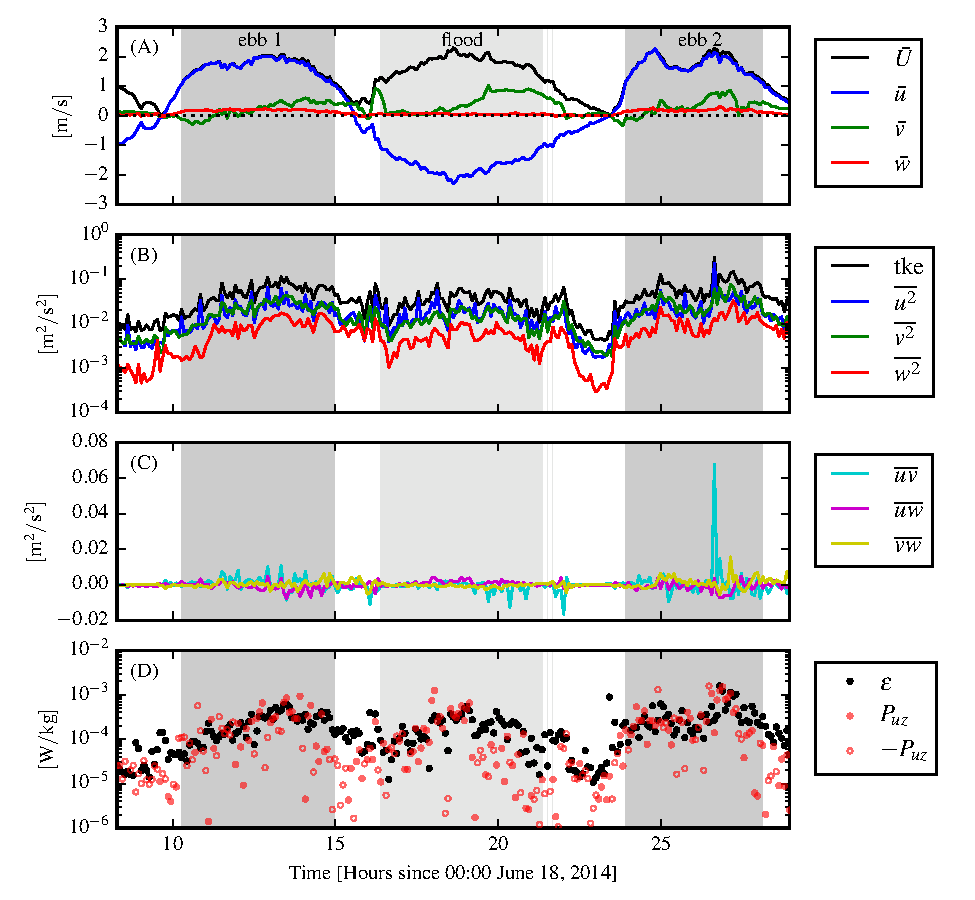
\includegraphics{TurbTime_TTM_01}
  \caption{Time series of mean velocities (A), turbulence energy and its components (B), Reynold's stresses (C), and turbulence dissipation rate (D) measured by the TTM during the June 2014 deployment. Shading indicates periods of ebb ($\bar{u}>1.0\ \mathrm{ms^{-1}}$, grey) and flood ($\bar{u}<-1.0\ \mathrm{ms^{-1}}$, lighter grey).}
  \label{fig:turbtime:ttm}
\end{figure*}

The previous section presented a comparison of $\vec{\bar{u}}$ measured by a TTM-mounted ADV to measurements from a co-located ADP. This comparison demonstrated that the IMU provides a reliable estimate of the ADV's orientation and that this can be utilized to estimate mean velocity in the Earth's reference frame. Turbulence velocity estimates from the same ADP are also in agreement with low-frequency TTM turbulence estimates (not shown), but the ADP does not resolve turbulence at the scales where motion contamination is strongest (0.1 to 1.0 Hz).

Ideally, moored motion-corrected turbulence velocity measurements would be validated against simultaneous independent validated measurements of turbulence velocity at the same scales and exact time and location. Accomplishing this, however, involves significant technical challenges that are not easily overcome---most notably the difficulty of measuring turbulence at the same point as the moving ADV. A slightly less ideal but much more realistic confirmation of the methodology might involve comparing the statistics of moored turbulence measurements to those from a nearby fixed platform, or a fixed platform placed at the same location at a different time \cite[e.g., the ``TTT" platform described in][]{Thomson++2012}. Unfortunately, to our knowledge, these measurements have not yet been made.

Lacking a relevant, fixed, independent turbulence measurement to compare to it is instructive to demonstrate the degree to which the moored measurements are consistent with turbulence theory and other turbulence measurements in similar flow environments. The previous section showed that the shape of the turbulence velocity spectra from moored ADVs is consistent with Kolmogorov's theory of locally isotropic turbulence, which has been observed consistently in turbulence measurements for decades \cite[]{Kolmogorov1941c,Grant++1962,McMillan++2016}. In particular, we observed an isotropic subrange---an $f^{-5/3}$ spectral slope and equal amplitude spectra between components---that is driven by anisotropic turbulence at longer timescales (Figures \ref{fig:spec:ttm}, \ref{fig:spec:sm}, \ref{fig:spec:torpedo}). This finding is interpreted as the first indication that the measurement systems presented are capable of accurately resolving turbulence. The degree to which uncorrected spectra were corrected toward this theoretical and observationally confirmed shape is interpreted as a measure of the improvement of the spectral estimates by motion correction.

Figure \ref{fig:turbtime:ttm} presents a time series of the mean velocity (A) and several turbulence statistics that were measured during the June 2014 TTM deployment. This figure shows the evolution of the flow through Admiralty Inlet during 1.5 tidal cycles. The $\tke$ (B), Reynold's stresses (C), dissipation, and one component of turbulence production (D) grow and strengthen with ebb or flood then subside during slack tide.  This component of turbulence production is:
\begin{align}
  \produz = \uw\frac{\partial \bar{u}}{\partial z} \qquad.
\end{align}
Where $\partial \bar{u}/\partial z$ is computed from the two ADVs on the TTM. The highest values of $\epsilon$ and $\produz$ occur at the peak of the ebb or flood, which is in agreement with other measurements in tidal channels. The agreement of the magnitude of $\produz$ with $\epsilon$ at those times suggests a local production-dissipation balance that is often observed in tidally forced channels \cite[]{Trowbridge++1999,Stacey++1999,McMillan++2016}. At other times, the value of $\produz$ is insufficient to balance $\epsilon$ or is negative. 

Inspection of the negative $\produz$ values reveals that most of them are caused by a reversed sign of $\uw$ rather than a reversed sign of $\partial u / \partial z$ (i.e., when compared to the sign of $u$). This finding suggests that uncertainty in $\uw$ may be contributing to discrepancies between $\produz$ and $\epsilon$. Furthermore, considering the complex nature of the bathymetry and shoreline at this site (i.e., the headland), it is not surprising that $\produz$ does not perfectly balance $\epsilon$. Other terms of the $\tke$ equation are likely to be important, such as turbulence advection, other components of production, and turbulent transport. The fact that the $\produz$ and $\epsilon$ terms are in near balance as often as they are indicates that bottom boundary layer physics are important to the turbulence dynamics at this site.

\begin{figure}[t]
  \centering
  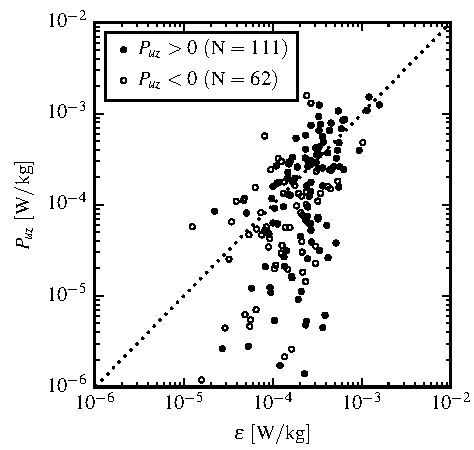
\includegraphics{EpsVProd01}
  \caption{$\produz$ vs. $\epsilon$ during the June 2014 TTM deployment for values of $|u|>1$ m/s. Values of negative production are indicated as open circles. }
  \label{fig:prodVeps}
\end{figure}

Figure \ref{fig:prodVeps} compares individual values of $\produz$ with $\epsilon$ directly. Given the assumptions implicit in this comparison and the discussion above, the degree of agreement between $\produz$ and $\epsilon$---especially for the highest values of $\epsilon$---suggests the turbulent boundary layer reaches the depth of these measurements (10 m) during the highest flow speeds. This result is further supported by a comparison of $\bar{U}$ with $\epsilon$ (Figure \ref{fig:epsVu}). Here we see a $\epsilon \propto \bar{U}^3$ dependence that is again suggestive of bottom boundary layer physics \cite[]{Trowbridge1992,Nash++2009}. At lower flow speeds, $\epsilon$ deviates from this relationship, which suggests that the boundary layer is no longer the dominant physical process at the depth of these measurements.

There are two intriguing differences between the ebb and flood datasets: 1) the drag coefficient relating $\epsilon$ to $\bar{U}^3$ is larger for ebbs, and 2) the fit does not hold as well for low flow speeds (Figure \ref{fig:epsVu}). These details are not surprising considering the complex bathymetry at the test site (Figure \ref{fig:map}). In particular, the flow immediately upstream of the measurement site is exposed to much more bathymetric curvature---i.e. from the headland---during ebb (when $\bar{u}$ is $>0$) than the during flood ($\bar{u}<0$). Based on this, one might expect flow separation (turbulence advection), turbulence production, or turbulence transport emanating from the headland to have a stronger impact on the flow at this site during ebb than flood. These effects are a likely contributor to the distinct relationships observed in Figure \ref{fig:epsVu}. 

The hypothesis that the headland is a key contributor to the turbulence dynamics at this site suggests that terms such as cross-stream turbulence advection, $\bar{v}\partial \tke / \partial y$, the lateral turbulent transport terms, $\partial \overline{u_iu_i v} / \partial y$, or lateral shear production, $\uv\partial \bar{u} / \partial y$, may contribute significantly to the dynamics of turbulence at this site. While we did not measure stratification profiles during these measurements, we do not typically expect buoyancy flux to play dominant role due to the fact that this region tends to be tidally well-mixed \cite[]{Geyer+Cannon1982}. In summary, bottom boundary layer physics seems to be the dominant process at the measurement site, with lateral advection, lateral transport, and lateral production of $\tke$ also potentially contributing---especially during ebb. A more detailed analysis of the turbulence and momentum dynamics of this headland is left for future work \cite[e.g., ][]{Warner++2013}.

\begin{figure*}[t]
  \centering
  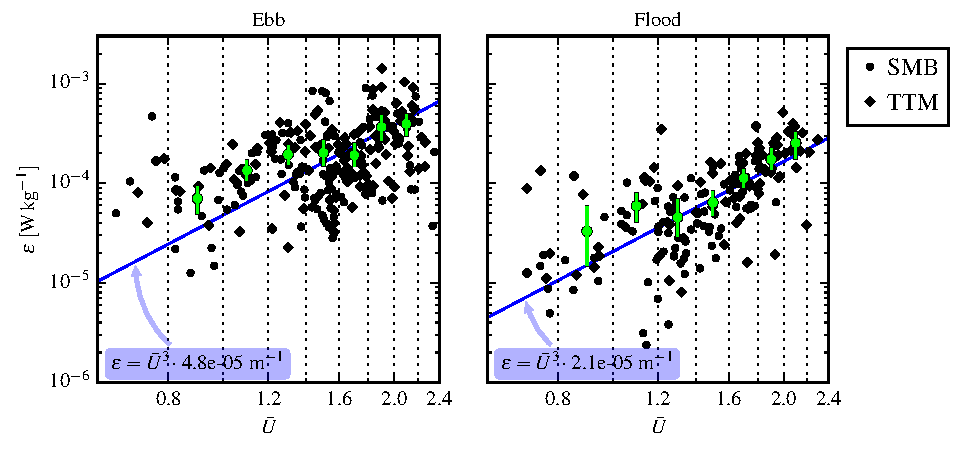
\includegraphics{EpsVU_03}
  \caption{A log-log plot of $\epsilon$ vs. $\bar{U}$ for the June 2014 TTM (diamonds) and May 2015 SMB (dots) deployments, during ebb (left) and flood (right). Black points are 5-minute averages.  Green dots are mean values within speed bins of 0.2 m s$^{-1}$ width that have at least 10 points (50 minutes of data); their vertical bars are 95\% bootstrap confidence intervals. The blue line shows a $U^3$ slope, wherein the proportionality constant (blue box) is calculated by taking the log-space mean of $\epsilon/U^3$. }
  \label{fig:epsVu}
\end{figure*}



%%% Local Variables:
%%% mode: latex
%%% TeX-master: "Kilcher_etal_IMU-ADV"
%%% End:
